%%%%%%%%%%%%%%%%%%%%%%%%%%%%%%%%%%%%%%%%%%%%%%%%%%%%%%%%%%%%%%%%%%%%%%
% Lớp 11 | Giới hạn. Hàm số liên tục | Hàm số liên tục
% Dạng 1D3?3-2: Tính liên tục thể hiện qua đồ thị
% Số câu: 19  (sinh tự động bởi tach_cau.py; từ nay thầy sửa trực tiếp file này)
%%%%%%%%%%%%%%%%%%%%%%%%%%%%%%%%%%%%%%%%%%%%%%%%%%%%%%%%%%%%%%%%%%%%%%

%%%%%%%%%%%%%%%% TRẮC NGHIỆM 4 PHƯƠNG ÁN %%%%%%%%%%%%%%%%

% nguồn: Ok_Toan11_TracNghiem_Lan2
\begin{ex}%[1D3N3-2]%[ma:4bd3b5d5]
	 \immini[thm]{Cho hàm số $y=f(x)$ có đồ thị như hình vẽ bên, trên khoảng $\left(-1;\,3 \right)$ hàm số gián đoạn tại điểm nào dưới đây?\\
	 \choice
		{\True  $x=1$}
		 {$x=0$}
		{$x=2$} 
		{$x=3$}}{ 
		\begin{tikzpicture}[scale=1,font=\normalsize,line join=round,line cap=round,>=stealth]
				\def\xmin{-3} \def\xmax{4} 
				\def\ymin{-1} \def\ymax{4.5} 
				\draw[->] (\xmin,0)--(0,0) node [below right]{$O$}-- (\xmax,0) node [below]{$x$}; 
				\draw[->] (0,\ymin)--(0,\ymax) node  [left]{$y$};
				\clip (\xmin+0.1,\ymin+0.1) rectangle  (\xmax-0.1,\ymax-0.1);
				\draw[smooth,samples=100,teal] plot[domain=-1.3:1](\x,{2*(\x)^2+1}); 
				\draw[smooth,samples=100,teal] (1,0)--(4,3) 
					(-1,2) node  [left]{$y=f (x)$};
				\draw[dashed]  (1,0)--(1,3)--(0,3);
				\draw[dashed] (2,0)--(2,1)--(0,1); 
				\coordinate [label = below:$1$] (B) at  (1,0);
				\coordinate [label =  below:$2$] (C) at (2,0);
				\coordinate  (D1) at (0,1);
				 \coordinate [label = left:$1$] (D) at (0,.8);
				\coordinate [label  = left:$3$] (E) at (0,3);
				 \coordinate (F) at (1,3);
				\coordinate (G)  at (2,1);
				\coordinate  (O) at (0,0);
				\foreach \x in {B,C,D1,E,F,G,O} \fill (\x) circle (1pt); 
			\end{tikzpicture}
		} 
	 \loigiai{
		Đồ thị bị \lq\lq  đứt\rq\rq\ tại điểm có hoành độ $x=1$ nên hàm số gián đoạn tại $x=1$.
	 }
\end{ex}

% nguồn: Ok_Toan11_TracNghiem_Lan2
\begin{ex}%[1D3N3-2]%[ma:6d5afb0e]
	\immini[thm]{Cho đồ thị của hàm số $y=f(x)$ như hình vẽ bên 
	Chọn mệnh đề  \textbf{sai}.
	\choice 
		{\True Hàm số $y=f(x)$ liên tục  tại điểm $x=1$}
		{Hàm số $y=f(x)$  liên tục tại điểm $x=0$}
		{Hàm số $y=f(x)$ liên tục tại điểm  $x=-1$}
		{Hàm số $y=f(x)$ liên tục tại điểm  $x=2$}}{
		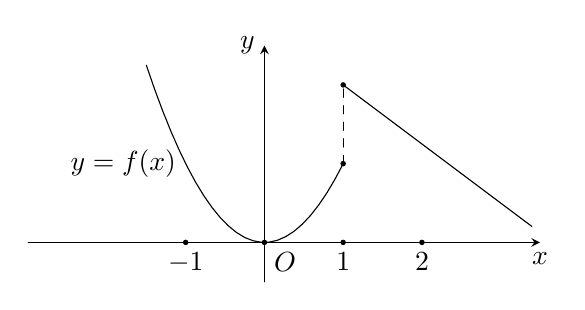
\begin{tikzpicture}[scale=1,font=\normalsize,line join=round,line cap=round,>=stealth]
				 \def\xmin{-3} \def\xmax{3.5}
				 \def\ymin{-.5} \def\ymax{2.5}
				\draw[->] (\xmin,0)--(0,0) node  [below right]{$O$}-- (\xmax,0) node [below]{$x$};
				\draw[->] (0,\ymin)--(0,\ymax) node  [left]{$y$};
				\clip (\xmin+0.1,\ymin+0.1) rectangle (\xmax-0.1,\ymax-0.1); 
				\draw plot[domain=-1.5:1](\x,{(\x)^2}); 
				 \draw (1,2)--(4,-.25)
					(-1,1) node [left]{$y=f  (x)$};
				\draw[dashed]  (1,1)--(1,2);
				\coordinate [label  = below:$-1$] (A) at (-1,0);
				\coordinate [label = below:$1$] (B) at  (1,0);
				 \coordinate [label = below:$2$] (C) at (2,0);
				\coordinate (O) at (0,0); 
				\coordinate  (E) at (1,1);
				\coordinate  (F) at (1,2);
				 \foreach \x in {A,B,C,O,E,F} \fill (\x) circle (1pt);
			\end{tikzpicture}
		} 
	 \loigiai{
		Nhìn vào đồ thị, ta thấy hàm số bị gián đoạn tại điểm $x=1$ nên nó không liên tục  tại $x=1$.
	} 
\end{ex}

% nguồn: Ok_Toan11_TracNghiem_Lan2
\begin{ex}%[1D3N3-2]%[ma:53c7ff1a]
	\immini{Hàm số $y=f(x)$ có đồ thị như hình bên. Hàm số gián đoạn tại điểm có hoành độ bằng bao nhiêu? 
	 \choice
		{\True $1$} 
		{$0$} 
		{$2$} 
		 {$3$}}{
		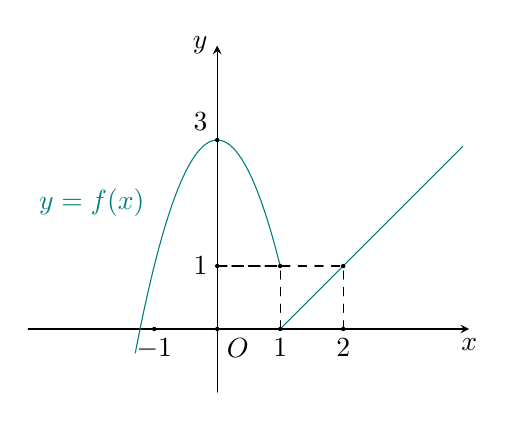
\begin{tikzpicture}[scale=0.8,font=\normalsize,line join=round,line cap=round,>=stealth]
				 \def\xmin{-3} \def\xmax{4}
				\def\ymin{-1} \def\ymax{4.5} 
				\draw[->] (\xmin,0)--(0,0) node  [below right]{$O$}-- (\xmax,0) node [below]{$x$};
				\draw[->] (0,\ymin)--(0,\ymax)  node [left]{$y$};
				\clip (\xmin+0.1,\ymin+0.1) rectangle (\xmax-0.1,\ymax-0.1); 
				\draw[smooth,samples=100,teal] plot[domain=-1.3:1](\x,{-2*(\x)^2+3}); 
				\draw[smooth,samples=100,teal] (1,0)--(4,3) 
					(-1,2) node [left]{$y=f (x)$}; 
				\draw[dashed]  (1,0)--(1,1)--(0,1);
				\draw[dashed]  (2,0)--(2,1)--(0,1);
				\coordinate [label =  below:$-1$] (A) at (-1,0);
				\coordinate [label =  below:$1$] (B) at (1,0);
				\coordinate [label = below:$2$]  (C) at (2,0);
				\coordinate [label = left:$1$]  (D) at (0,1);
				\coordinate [label = above left:$3$]  (E) at (0,3);
				\coordinate  (F) at (1,1);
				 \coordinate (O) at (0,0);
				\coordinate (G)  at (2,1);
				\foreach \x in {A,B,C,D,E,F,G,O} \fill (\x)  circle (1pt);
			\end{tikzpicture}
		} 
	\loigiai{ 
		DĐồ thị bị \lq\lq đứt\rq\rq\, tại điểm có hoành độ $x=1$ nên nó gián  đoạn tại $x=1$.
	 }
\end{ex}

% nguồn: Ok_Toan11_TracNghiem_Lan2
\begin{ex}%[1D3N3-2]%[ma:a19b9c7e]
	\immini[thm]{Cho hàm số $y=f(x)$ có đồ thị như hình  bên. Hàm số $y=f(x)$ không liên tục tại
	 \choice
		{$x=0$} 
		 {\True $x=2$}
		 {$x=1$}
		{$x=4$}}{ 
		\begin{tikzpicture}[line join = round,line cap = round,>=stealth,x = 1cm,y = 1cm,scale=0.7]
				 \def\xmin{-2.5} \def\xmax{4.5}
				\def\ymin{-2.5} \def\ymax{2.5} 
				\def\hamso{(1)/((\x)-2)} 
				 \pgfmathsetmacro{\tiemcanngang}{0}
				 \draw[->] (\xmin,0)--(0,0) node[above left]{$O$}--(\xmax,0) node[below]{$x$};
				\draw[->]  (0,\ymin)--(0,\ymax) node[right]{$y$};
				\fill (0,0) circle (1pt); 
				\begin{scope}
					\clip (\xmin,\ymin) rectangle  (\xmax,\ymax);
					\draw[samples=300,domain=\xmin:1.9,smooth,orange] plot  (\x,{\hamso});
					\draw[samples=300,domain=2.01:\xmax,smooth,orange] plot (\x,{\hamso}); 
				\end{scope}
				 \draw[dashed](\xmin,\tiemcanngang)--(\xmax,\tiemcanngang);
				 \draw[dashed](2,\ymin)--(2,\ymax);
				\coordinate [label  = below:$1$] (B) at (1,0);
				\coordinate [label  = below right:$2$] (C) at (2,0);
				\foreach \x  in {B,C} \fill (\x) circle (1pt);
			\end{tikzpicture}
		 }
	 \loigiai{
		Vì $\heva{&\lim\limits_{x \to 2^+}f(x)=+\infty \\ 
		&\lim\limits_{x \to 2^-}f(x)=-\infty}$ nên hàm số không liên tục  tại $x=2$.
	} 
\end{ex}

% nguồn: Ok_Toan11_TracNghiem_Lan2
\begin{ex}%[1D3N3-2]%[ma:d91c8e11]
	\immini[thm]{Cho hàm số $f(x)$ có đồ thị như hình vẽ. Chọn khẳng định \textbf{sai} trong các  khẳng định dưới đây
	 \choice
		{Hàm số $f(x)$ liên tục  tại $x=1$}
		{Hàm số $f(x)$  liên tục trên khoảng$\left(-3;\,-2 \right)$}
		{Hàm số $f(x)$ gián đoạn tại  $x=-1$}
		{\True Hàm số  $f(x)$ liên tục trên khoảng$\left(-3;\,2 \right)$}}{
		\begin{tikzpicture}[scale=0.7,font=\normalsize,line join=round,line cap=round,>=stealth]
				 \def\xmin{-4} \def\xmax{2.5}
				\def\ymin{-5} \def\ymax{2.5} 
				\draw[->] (\xmin,0)--(0,0) node  [below right]{$O$}-- (\xmax,0) node [below]{$x$};
				\draw[->] (0,\ymin)--(0,\ymax) node  [left]{$y$};
				\clip (\xmin+0.1,\ymin+0.1) rectangle (\xmax-0.1,\ymax-0.1); 
				 \draw plot[domain=-1:1.5](\x,{(\x)^2+2*(\x)-3});
				 \draw (-3,2)--(-1,-1)
					(0,1.5) node [left]{$y=f  (x)$};
				\draw[dashed](-1,-1)--(-1,-4); 
				\coordinate [label = below:$-1$] (A) at (-1,0); 
				 \coordinate [label = below right:$1$] (B) at (1,0);
				\coordinate (C) at (0,0); 
				\coordinate [label = right:$-3$] (D) at (0,-3); 
				\coordinate (E) at  (-1,-1);
				\coordinate (F)  at (-1,-4);
				\coordinate [label = right:$-4$] (G) at (0,-4); \coordinate [label =  left:$-2$] (H) at (0,-2);
				\foreach \x  in {A,B,C,D,E,F,G,H} \fill (\x) circle (1pt);
			\end{tikzpicture}
		 }
	\loigiai{ 
		Quan sát đồ  thị ta thấy $\lim\limits_{x \to 1^-}f(x)=\lim\limits_{x \to 1^+}f(x)=f\left(1\right)=0$, do đó hàm số liên tục tại $x=1$.\\
		Lại có, $\lim\limits_{x \to -1^-}f(x)=-2$;  $\lim\limits_{x \to -1^+}f(x)=-4$.\\
		Suy ra $\lim\limits_{x \to  -1^+}f(x)\ne \lim\limits_{x \to -1^-}f(x)$ nên $\lim\limits_{x \to -1}f(x)$ không tồn tại. Do đó hàm số gián đoạn tại $x=-1$.\\
		Mà $-1\in \left(-3;\,2 \right)$ nên hàm số không thể liên  tục trên khoảng $\left(-3;\,2 \right)$.
	 }
\end{ex}

% nguồn: Ok_TracNghiemLop11_Lan1
\begin{ex}%[1D3N3-2]%[ma:b9930120]
	 \immini{
	Cho hàm số $y=f(x)$ có đồ thị như hình vẽ bên. Trên đoạn $[-2;3]$ hàm số gián đoạn tại điểm có hoành độ bao  nhiêu?
	\choice 
		 {\True $-1$}
		 {$0$}
		 {$1$}
		{$2$} 
		 }{
		\begin{tikzpicture}[line cap=round,line join=round,>=stealth]
				 \draw[->] (-3,0) -- (4,0);
				\draw[->] (0,-1)  -- (0,6);
				\clip  (-3,-1) rectangle (4.5,5.7);
				 \draw[smooth,samples=100,domain=-1:1] plot (\x,{(\x+1)^2+1});
				\draw [->]  (-3,2)-- (-1,0);
				\draw (1,5)-- (2,1) (3.5,4)-- (2,1); 
				\draw [dashed] (-1,0) --  (-1,1)--(2,1)--(2,0)
					(0,5)--(1,5)--(1,0) 
					 (-2,0)--(-2,1)
					(3,0)--(3,3); 
				\begin{normalsize}
					\draw (4,0.3)  node {$x$};
					\draw  (-0.3,5.5) node{$y$};
					 \draw (-0.3,5) node[left] {$5$};
					\draw (0.3,-0.3) node  {$O$};
					\draw (1,-0.3) node[below] {$1$}; 
					\draw  (2,-0.3) node[below] {$2$};
					 \draw (-1,-0.3) node[below] {$-1$};
					 \draw (-2,-0.3) node[below] {$-2$};
					\draw (3,-0.3) node[below]  {$3$};
					\draw  (0,1) node[below left] {$1$};
				\end{normalsize}
			\end{tikzpicture}
		} 
	\loigiai{ 
		Quan sát đồ thị ta thấy $\heva{&  \lim\limits_{x \rightarrow -1^{-}} f(x)=0\\ &\lim\limits_{x \rightarrow -1^{+}} f(x)=1.}$\\
		Vì $\lim\limits_{x \rightarrow -1^-} f(x) \neq \lim\limits_{x \rightarrow -1^{+}}  f(x)$ nên $\lim\limits_{x \rightarrow -1} f(x)$ không tồn tại.\\
		 Do đó hàm số gián đoạn tại $x=-1$.
	 }
\end{ex}

% nguồn: Ok_TracNghiemLop11_Lan1
\begin{ex}%[1D3N3-2]%[ma:304cf1f0]
	\immini[thm]{Cho  hàm số $y=f(x)$ có đồ thị như hình vẽ bên. Khẳng định nào sau đây đúng?
	\choice 
		{\True $y=f(x)$ liên  tục trên các khoảng $(-\infty;1)$ và $(1;+\infty)$}
		{$y=f(x)$ liên tục trên  khoảng $(0;+\infty)$}
		{$y=f(x)$ liên tục  trên khoảng $(-\infty;2)$}
		 {$y=f(x)$ liên tục trên $\mathbb{R}$}
		}{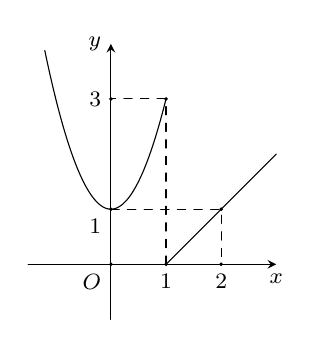
\begin{tikzpicture}[line join = round,line cap = round,>=stealth,font=\footnotesize,scale=0.7]
		\draw[->] (-1.5,0)--(3,0) node[below]{$x$}; 
		 \draw[->] (0,-1)--(0,4) node[left]{$y$};
		\fill (0,0) circle (1pt)  node[below left]{$O$};
		\draw (1,0)--(3,2); 
		\draw[samples=100,domain=-1.2:1,smooth] plot (\x,{2*(\x)^2+1}); 
		\fill (1,0) node[below] {$1$} circle  (1pt);
		\fill (0,1) node[below left] {$1$} circle (1pt); 
		\fill (0,3) node[left] {$3$}  circle (1pt);
		\fill (2,0) node[below] {$2$}  circle (1pt);
		 \fill (1,3) circle (1pt);
		\fill  (2,1) circle (1pt);
		 \draw[dashed] (1,0)--(1,3)--(0,3)
			 (0,1)--(2,1)--(2,0);
	\end{tikzpicture}
		} 
	 \loigiai{
		Dựa vào đồ  thị, ta thấy hàm số $y=f(x)$ liên tục trên các khoảng $(-\infty;1)$ và $(1;+\infty)$.
	} 
\end{ex}

% nguồn: Ok_TracNghiemLop11_Lan1
\begin{ex}%[1D3N3-2]%[ma:19edd384]
	\immini{ Hàm số $f(x)$ có đồ thị như hình bên  dưới không liên tục tại điểm có hoành độ là bao nhiêu?
	 \choice
		 {$x=0$}
		 {\True $x=1$}
		 {$x=2$}
		{$x=3$}}{\begin{tikzpicture}[scale=0.8,font=\footnotesize,line join=round,line cap=round,>=stealth]
		\draw[->]  (-2.1,0)--(5.1,0) node[below left] {$x$};
		\draw[->]  (0,-1.1)--(0,5.1) node[below left] {$y$};
		\draw (0,0)  node [below left] {$O$};
		\foreach  \x/\nx in {1/1,2/2}
		\draw[thin] (\x,1pt)--(\x,-1pt)  node [below] {$\nx$};
		 \foreach \y/\ny in {1/1,3/3}
		\draw[thin] (1pt,\y)--(-1pt,\y) node [left] {$\ny$}; 
		 \draw[dashed](1,0)--(1,3)--(0,3);
		\draw[dashed](2,0)--(2,1)--(0,1); 
		\begin{scope}
			\clip (-2,-1)  rectangle (5,5);
			\draw[samples=200,domain=1:-2,smooth,variable=\x] plot  (\x,{2*(\x)^2+1});
			\draw[samples=200,domain=5:1,smooth,variable=\x] plot  (\x,{(\x)-1});
		\end{scope}
	\end{tikzpicture}
		 }
	 \loigiai{
		Dựa vào đồ thị, ta thấy $\heva{&\lim\limits_{x\to 1^+}f(x)=0\\&\lim\limits_{x\to 1^-}f(x)=3}$  nên hàm số $f(x)$ gián đoạn tại $x=1$.
	 }
\end{ex}

% nguồn: Ok_TracNghiemLop11_Lan1
\begin{ex}%[1D3N3-2]%[ma:ec281384]
	Hình nào trong các hình dưới đây là đồ thị của  hàm số không liên tục tại $x=-1$?
	\choice 
		{\begin{tikzpicture}[line join=round,line cap=round,>=stealth]
		 \tikzset{every node/.style={scale=0.9}}
		\draw[->] (-2.1,0)--(1.6,0) node[below left] {$x$}; 
		\draw[->] (0,-1.1)--(0,2.1) node[below  left] {$y$};
		\draw (0,0) node [below left]  {$O$};
		\foreach \x/\nx in {-1/-1,1/1} 
		\draw[thin] (\x,1pt)--(\x,-1pt) node  [below] {$\nx$};
		\foreach \y/\ny in  {1/1}
		\draw[thin] (1pt,\y)--(-1pt,\y)  node [left] {$\ny$};
		\begin{scope}
			 \clip (-2,-2) rectangle (2,2);
			\draw[samples=200,domain=-1.5:0.6,smooth,variable=\x]  plot (\x,{1*(\x)+1});
		\end{scope}
	\end{tikzpicture}
		 }
		{\begin{tikzpicture}[line join=round,line cap=round,>=stealth]
		 \tikzset{every node/.style={scale=0.9}}
		\draw[->] (-2.8,0)--(1,0) node[below  left] {$x$};
		\draw[->]  (0,-1)--(0,2.1) node[below left] {$y$};
		\draw (0,0)  node [below left] {$O$};
		 \foreach \x/\nx in {-1/-1}
		\draw[thin] (\x,1pt)--(\x,-1pt)  node [below] {$\nx$};
		\foreach  \y/\ny in {1/1}
		\draw[thin] (1pt,\y)--(-1pt,\y) node [left]  {$\ny$};
		\begin{scope}
			\clip (-2.7,-1.6) rectangle (1.6,2); 
			\draw[samples=200,domain=-2.5:0.5,smooth,variable=\x] plot  (\x,{1*(\x)^2+2*(\x)+1});
		\end{scope}
	\end{tikzpicture}
		 }
		{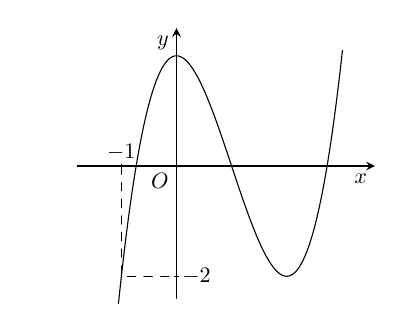
\begin{tikzpicture}[line join=round,line cap=round,>=stealth,scale=0.7]
		\tikzset{every  node/.style={scale=0.8}}
		\draw[->] (-1.8,0)--(3.6,0) node[below left]  {$x$};
		\draw[->]  (0,-2.4)--(0,2.5) node[below left] {$y$};
		\draw  (0,0) node [below left] {$O$};
		\foreach \x/\nx in  {-1/-1}
		 \draw[thin] (\x,1pt)--(\x,-1pt) node [above] {$\nx$};
		\foreach \y/\ny in  {-2/-2}
		\draw[thin] (1pt,\y)--(-1pt,\y) node [right] {$\ny$}; 
		\draw[dashed](-1,0)--(-1,-2)--(0,-2); 
		\begin{scope}
			\clip (-2.7,-2.5) rectangle (3.6,2.1); 
			\draw[samples=200,domain=-2:3.6,smooth,variable=\x] plot (\x,{1*(\x)^3-3*(\x)^2+2}); 
		\end{scope}
	\end{tikzpicture}
		 }
		{\True \begin{tikzpicture}[line join=round,line cap=round,>=stealth,scale=0.7]
		\tikzset{every  node/.style={scale=0.8}}
		 \draw[->] (-2.1,0)--(1.6,0) node[below left] {$x$};
		\draw[->] (0,-2.4)--(0,2.5)  node[below left] {$y$};
		\draw (0,0)  node [below left] {$O$};
		\foreach \x/\nx in {-1/-1} 
		\draw[thin] (\x,1pt)--(\x,-1pt) node  [below left] {$\nx$};
		\foreach \y/\ny in {-2/-2,1/1} 
		 \draw[thin] (1pt,\y)--(-1pt,\y) node [right] {$\ny$};
		 \draw[dashed](-1,0)--(-1,1)--(0,1);
		\begin{scope}
			\clip (-2.7,-2.5) rectangle  (3.6,2.1);
			\draw[samples=200,domain=-1:3.6,smooth,variable=\x]  plot (\x,{1*(\x)^3+3*(\x)^2-2});
			 \draw (-2,2)--(-1,1);
		\end{scope}
	\end{tikzpicture}
		 }
	 \loigiai{
		Xét  đồ thị
		\begin{center}
			\begin{tikzpicture}[>=stealth,x=1cm,y=1cm,scale=0.6]
					\draw[->,black]  (-2.2,0) -- (4,0) node[below] {$x$};
					\foreach \x in{-2,3} \draw[xshift=\x cm] (0pt,-2pt)--(0pt,2pt); 
					\draw[->,black]  (0,-2.5) -- (0,3.5) node[left] {$y$};
					\foreach \y  in{-2,-1,2,3} \draw[yshift=\y cm] (-2pt,0pt)--(2pt,0pt);
					\draw [-,black](-1,-2.5)--(-1,3.5); 
					 \draw (1,0) node[below]{$1$} circle (1pt);
					\draw (2,0) node[below]{$2$} circle  (1pt);
					\draw (-1,0) node[above left]{$-1$} circle  (1pt);
					\draw (0,1) node[left]{$1$} circle (1pt); 
					\draw (0,0) node[below right]{$O$} circle  (1pt);
					\draw [dashed] (1,0)--(1,1)--(0,1); 
					\draw[smooth,samples=100,domain=-0.8:3]  plot (\x,{ln((\x)+1)/ln(2)});
				\end{tikzpicture}0
		\end{center}
		Ta suy  ra $\lim\limits_{x\to -1^-}f(x)=1$ và $\lim\limits_{x\to -1^+}f(x)=0$.\\
		Suy ra $\lim\limits_{x\to -1^-}f(x)\ne  \lim\limits_{x\to -1^+}f(x)$.
	 }
\end{ex}

% nguồn: Ok_TracNghiemLop11_Lan1
\begin{ex}%[1D3N3-2]%[ma:b9f54b9a]
	\immini{ 
	Cho đồ  thị hàm số $y=f(x)$ có đồ thị như hình vẽ bên. Chọn mệnh đề đúng trong các mệnh đề sau
	\choice 
		{Hàm số $y=f(x)$ gián đoạn  tại $x_0 = 0$}
		{$\displaystyle\lim\limits_{x \rightarrow +\infty} f\left(x\right)  = -1$}
		{$\displaystyle\lim\limits_{x  \rightarrow -\infty} f\left(x\right) = -1$}
		{\True Hàm số $y=f(x)$ liên tục trên $\mathbb{R}$}}{ 
		\begin{tikzpicture}[>=stealth,scale=0.8]
				\draw[->] (-2,0)--(0,0)  node[below left]{$O$}--(4,0) node[above]{$x$};
				\draw[->,color=black]  (0,-2)--(0,4) node[right]{$y$};
				\clip (-3,-3) rectangle  (4,4);
				\draw (-2,-2)--(-0.5,1.2)--(0,0)--(1.5,3.2)--(3.9,-2)  node[left]{$y=f (x)$};
				 \draw[dashed] (-2,-1)--(4,-1);
				\draw[fill] (0,-1) circle (1.3pt) node[below  left]{$-1$};
				\draw[fill]  (-1.05,0) circle (1.3pt) node[above left]{$-1$};
			\end{tikzpicture}
		 }
	\loigiai{ 
		Quan sát đồ  thị hàm số, ta có
		\begin{enumerate}[$\bullet$]
			\item Đồ thị hàm số là các đường liền nét trên khoảng $\left(-\infty;+\infty\right)$  do đó hàm số liên tục trên $\mathbb{R}$.
			\item $\displaystyle\lim\limits_{x  \rightarrow +\infty} f\left(x\right) = -\infty$.
			 \item $\displaystyle\lim\limits_{x \rightarrow -\infty} f\left(x\right) = -\infty$.
		\end{enumerate}
	} 
\end{ex}

% nguồn: Ok_Toan11_TracNghiem_Lan2
\begin{ex}%[1D3H3-2]%[ma:d663ed8e]
	Hình nào trong các hình dưới đây là đồ thị của  hàm số \textbf{không} liên tục tại $x=1$?
	\choice 
		{ \begin{tikzpicture}[line join = round,line cap = round,>=stealth,scale=0.5]
		\draw[->] (-2.5,0)--(0,0) node[below left]{$O$}--(2.5,0)  node[below]{$x$};
		\draw[->]  (0,-1.5)--(0,3.5) node[right]{$y$};
		\draw[samples=200,domain=-1.2:3.5,smooth,blue] plot (\x,{abs (\x-1) + 1}) node[below  right]{$ $};
		\draw[dashed](1,0)--(1,1)--(0,1); 
		 \node[below] at (1,0){${1}$};
		 \node[left] at (0,1){${1}$};
		\fill (1,0) circle  (1pt);
		 \fill (0,1) circle (1pt);
		\fill (1,1)  circle (1pt);
		\fill (0,0) circle (1pt); 
	\end{tikzpicture}
		 }
		{ 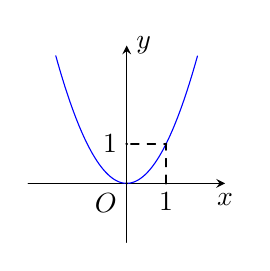
\begin{tikzpicture}[line join = round,line cap = round,>=stealth,scale=0.5]
		\draw[->]  (-2.5,0)--(0,0) node[below left]{$O$}--(2.5,0) node[below]{$x$};
		\draw[->] (0,-1.5)--(0,3.5) node[right]{$y$}; 
		\draw[samples=200,domain=-1.8:1.8,smooth,blue]  plot (\x,{(\x)^2}) node[below right]{$ $};
		 \draw[dashed](1,0)--(1,1)--(0,1);
		\node[below]  at (1,0){${1}$};
		 \node[left] at (0,1){${1}$};
		\fill (1,0) circle  (1pt);
		 \fill (0,1) circle (1pt);
		 \fill (1,1) circle (1pt);
		\fill (0,0) circle (1pt); 
	\end{tikzpicture}
		} 
		{ 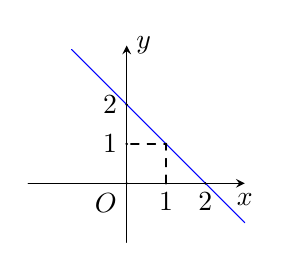
\begin{tikzpicture}[line join = round,line cap = round,>=stealth,scale=0.5]
		\draw[->] (-2.5,0)--(0,0) node[below left]{$O$}--(3,0)  node[below]{$x$};
		\draw[->] (0,-1.5)--(0,3.5) node[right]{$y$}; 
		\draw[samples=200,domain=-1.4:3,smooth,blue] plot (\x,{2-(\x)})  node[below right]{$ $};
		 \draw[dashed](1,0)--(1,1)--(0,1);
		\node[below]  at (1,0){${1}$};
		\node[below]  at (2,0){${2}$};
		\node[left] at  (0,1){${1}$};
		\node[left] at  (0,2){${2}$};
		\fill (1,0) circle (1pt); 
		\fill (0,1)  circle (1pt);
		\fill (1,1)  circle (1pt);
		 \fill (0,0) circle (1pt);
		\fill (0,2)  circle (1pt);
		\fill (2,0) circle (1pt); 
	\end{tikzpicture}
		 }
		{\True 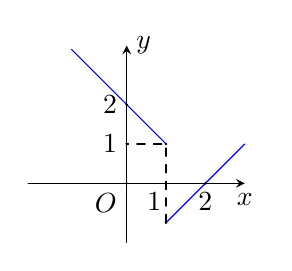
\begin{tikzpicture}[line join = round,line cap = round,>=stealth,scale=0.5]
		 \draw[->] (-2.5,0)--(0,0) node[below left]{$O$}--(3,0) node[below]{$x$};
		\draw[->] (0,-1.5)--(0,3.5) node[right]{$y$}; 
		\draw[samples=200,domain=-1.4:1,smooth,blue] plot (\x,{2-(\x)}) node[below right,blue]{$  $};
		\draw[samples=200,domain=1:3,smooth,blue] plot (\x,{-2+(\x)}) node[below right]{$ $}; 
		\draw[dashed](1,-1)--(1,1)--(0,1); 
		\node[below]  at (0.7,0){${1}$};
		\node[below] at (2,0){${2}$}; 
		 \node[left] at (0,1){${1}$};
		\node[left] at (0,2){${2}$}; 
		\fill (1,0) circle (1pt); 
		\fill (0,1)  circle (1pt);
		\fill (1,1) circle  (1pt);
		 \fill (0,0) circle (1pt);
		\fill  (0,2) circle (1pt);
		\fill  (2,0) circle (1pt);
		\fill (1,-1) circle  (1pt);
	\end{tikzpicture}
		 }
	 \loigiai{
		Đồ thị bị \lq\lq đứt\rq\rq\, tại điểm có hoành độ $x=1$ nên  nó không liên tục tại $x=1$.
	} 
\end{ex}

% nguồn: Ok_TracNghiemLop11_Lan1
\begin{ex}%[1D3K3-2]%[ma:0c9e6ae2]
	Cho cấp số cộng $({{u}_{n}})$ thỏa mãn $\heva{ 
	 & {{u}_{1}}+{{u}_{7}}=26 \\
	& {{u}_{2}}^2+{{u}_{6}}^2=466  \\
	}$. Mệnh đề nào sau  đây đúng?
	\choice 
		{ $\heva{ 
		&  {{u}_{1}}=13 \\
		 & d=-3 \\
		 }$}
		{  $\heva{
		&  {{u}_{1}}=10 \\
		& d=-3  \\
		}$} 
		{  \True $\heva{
		 & {{u}_{1}}=1 \\
		 & d=4 \\
		 }$}
		{  $\heva{
		&  {{u}_{1}}=13 \\
		 & d=-4 \\
		 }$}
	\loigiai{ 
		Ta có 
		 $$\heva{
		& {{u}_{1}}+{{u}_{7}}=26  \\
		&  {{u}_{2}}^2+{{u}_{6}}^2=466
		} 
		\Leftrightarrow \heva{ 
		 & 2{{u}_{1}}+6d=26 \\
		 & {{({{u}_{1}}+d)}^2}+{{({{u}_{1}}+5d)}^2}=466 \\
		}\Leftrightarrow \heva{ 
		 & {{u}_{1}}=13-3d \quad (1) \\
		&  {{({{u}_{1}}+d)}^2}+{{({{u}_{1}}+5d)}^2}=466.\quad(2)
		 }$$
		Thay (1) vào  (2) ta được
		{\allowdisplaybreaks 
		\begin{eqnarray*}
			(13-2d)^2+(13+2d)62=466\Leftrightarrow 8d^2+338=466\Leftrightarrow \hoac{&d=4\Rightarrow u_1=1\\&d=-4\Rightarrow u_1=25.} 
		\end{eqnarray*}
		} 
	} 
\end{ex}

% nguồn: Ok_TracNghiemLop11_Lan1
\begin{ex}%[1D3B3-2]%[ma:6355112c]
	Một cấp số cộng có $6$ số hạng. Biết rằng tổng của số hạng đầu và số hạng cuối bằng $17;$ tổng của số hạng thứ hai và số hạng thứ  tư bằng $14$. Tìm công sai $d$ của câp số cộng đã cho.
	\choice 
		{ $d=2$ } 
		{ $d=5$ } 
		{ \True $d=-3$ } 
		 { $d=4$ }
	 \loigiai{Ta có
		 $\heva{
		& {{u}_{1}}+{{u}_{6}}=17  \\
		 & {{u}_{2}}+{{u}_{4}}=14 \\
		}\Leftrightarrow  \heva{
		 & 2{{u}_{1}}+5d=17 \\
		&  2{{u}_{1}}+6d=14 \\
		 }\Leftrightarrow \heva{
		& {{u}_{1}}=16  \\
		& d=-3.  \\
	}$} 
\end{ex}

% nguồn: Ok_TracNghiemLop11_Lan1
\begin{ex}%[1D3B3-2]%[ma:280d4baf]
	Trong các dãy số được cho dưới đây, dãy số nào {\bf không}  phải là cấp số cộng?
	\choice 
		{ ${{u}_{n}}=-{{2}^{n}}+15$} 
		{ ${{u}_{n}}=-4n+9$} 
		 { ${{u}_{n}}=-2n-21$}
		 { \True ${{u}_{n}}=-2n+19$}
	\loigiai{ 
	Dãy số ${{u}_{n}}=-{{2}^{n}}+15$ không có dạng $an+b$ nên có không  phải là cấp số cộng.}
\end{ex}

% nguồn: Ok_TracNghiemLop11_Lan1
\begin{ex}%[1D3B3-2]%[ma:999cf900]
	 Cho cấp số cộng $({{u}_{n}})$ có ${{u}_{3}}=15$ và $d=-2$. Tìm ${{u}_{n}}$
	 \choice
		{ ${{u}_{n}}=\dfrac{3}{2}{{n}^2}-4$} 
		{ ${{u}_{n}}=-3n-17$} 
		{ \True  ${{u}_{n}}=-2n+21$}
		{  ${{u}_{n}}=-\dfrac{3}{2}n+12$}
	\loigiai{ 
		Ta có $\heva{ 
		&  15={{u}_{3}}={{u}_{1}}+2d \\
		 & d=-2 \\
		}\Leftrightarrow  \heva{
		 & {{u}_{1}}=19 \\
		 & d=-2 \\
	}\Rightarrow  {{u}_{n}}={{u}_{1}}+(n-1)d=-2n+21$.}
\end{ex}


%%%%%%%%%%%%%%%% ĐÚNG/SAI %%%%%%%%%%%%%%%%

% nguồn: Ok_dungsai_lop11_Lan1
\begin{ex}%[1D3H3-2]%[ma:d88370ab]
 Cho bốn đồ thị của ba hàm số ở hình dưới đây. Hãy cho biết tính đúng  sai của mỗi nhận xét về các hàm số?
 \begin{center}
  \begin{tabular}{cccc}
   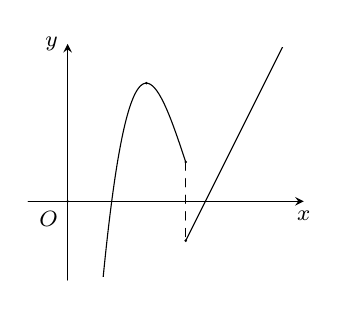
\begin{tikzpicture}[line join = round,line cap = round,>=stealth,font=\footnotesize,scale=0.5]
     \def\xt{-1} \def\xp{6} \def\yd{-2} \def\yt{4} 
     \def\a{1} 
     \def\b{-9} 
     \def\c{24} 
     \def\d{-17} 
     \draw[->]  (\xt,0)--(\xp,0) node[below]{$x$};
      \draw[->] (0,\yd)--(0,\yt) node[left]{$y$};
     \fill (0,0) circle  (1pt) node[below left]{$O$};
     \begin{scope}
      \clip (\xt+0.1,\yd+0.1) rectangle (\xp-0.1,\yt-0.1); 
      \draw[samples=150,smooth,domain=\xt:3] plot  (\x,{\a*(\x)^3+(\b)*(\x)^2+(\c)*\x+(\d)});
       \draw[samples=150,smooth,domain=3:\xp] plot (\x,{2*(\x)-7});
     \end{scope}
     \foreach \x/\y  in {2/3,3/1,3/-1}
      { 
      \fill (\x,\y) circle (1pt);
      }
      \draw[dashed] (3,1)--(3,-1);
    \end{tikzpicture}
   &\begin{tikzpicture}[>=stealth,line join=round,line cap=round,font=\normalsize,scale=0.5]
  \draw[->] (-2,0) -- (5,0) node[below] {\scriptsize  $x$};
   \draw[->] (0,-2) -- (0,5) node[left] {\scriptsize $y$};
  \draw (0,0) node[above left]{\scriptsize  $O$}
   (1,0)  node[below]{$1$};
  \clip  (-2,-2) rectangle (5,5);
  \draw[smooth,samples=200,domain=-2:1]  plot (\x,{(\x)^2-2*(\x)+1});
   \draw[smooth,samples=200,domain=1:5] plot (\x,{(\x)-1});
  \draw[fill] (0,0) circle (1pt); 
 \end{tikzpicture}
   &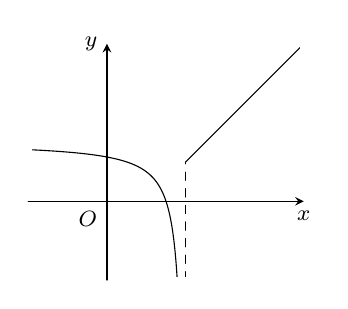
\begin{tikzpicture}[line join = round,line cap = round,>=stealth,font=\footnotesize,scale=0.5]
  \def\xt{-2} \def\xp{5} \def\yd{-2} \def\yt{4} 
   \def\a{6}
   \def\b{-9}
  \def\c{4} 
  \def\d{-8} 
  \draw[->] (\xt,0)--(\xp,0) node[below]{$x$}; 
   \draw[->] (0,\yd)--(0,\yt) node[left]{$y$};
  \fill  (0,0) circle (1pt) node[below left]{$O$};
  \pgfmathsetmacro{\tcn}{(\a)/(\c)} 
   \pgfmathsetmacro{\tcd}{-(\d)/(\c)}
  \begin{scope}
   \clip (\xt+0.1,\yd+0.1)  rectangle (\xp-0.1,\yt-0.1);
   \draw[dashed]  (\tcd,\yd)--(\tcd,\tcd-1);
   \draw[samples=150,smooth,domain={\tcd}:\xp] plot  (\x,\x-1);
   \draw[samples=150,smooth,domain=\xt:{\tcd-0.01}] plot  (\x,{(\a*\x+(\b))/(\c*\x+(\d))});
  \end{scope}
 \end{tikzpicture}
   & 
   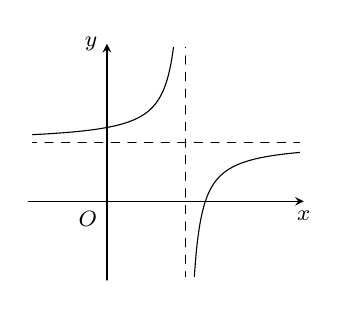
\begin{tikzpicture}[line join = round,line cap = round,>=stealth,font=\footnotesize,scale=0.5]
     \def\xt{-2} \def\xp{5}  \def\yd{-2} \def\yt{4}
     \def\a{6} 
      \def\b{-15}
      \def\c{4}
     \def\d{-8} 
     \draw[->]  (\xt,0)--(\xp,0) node[below]{$x$};
     \draw[->]  (0,\yd)--(0,\yt) node[left]{$y$};
     \fill (0,0) circle (1pt)  node[below left]{$O$};
      \pgfmathsetmacro{\tcn}{(\a)/(\c)}
     \pgfmathsetmacro{\tcd}{-(\d)/(\c)} 
     \begin{scope}
       \clip (\xt+0.1,\yd+0.1) rectangle (\xp-0.1,\yt-0.1);
      \draw[dashed] (\xt,\tcn)--(\xp,\tcn) 
      (\tcd,\yd)--(\tcd,\yt); 
       \draw[samples=150,smooth,domain={\tcd+0.01}:\xp] plot (\x,{(\a*\x+(\b))/(\c*\x+(\d))});
      \draw[samples=150,smooth,domain=\xt:{\tcd-0.01}] plot  (\x,{(\a*\x+(\b))/(\c*\x+(\d))});
     \end{scope}
    \end{tikzpicture}
   \\ 
   Đồ thị $y=f(x)$ &Đồ thị $y=g(x)$&  Đồ thị $y=h(x)$ &Đồ thị $y=k(x)$
  \end{tabular}
 \end{center}
  \choiceTF
  {Hàm số $y=f(x)$ liên tục trên tập xác định của nó} 
  {\True Hàm số $y=g(x)$ liên tục trên tập  xác định của nó}
  {\True  Hàm số $y=h(x)$ không liên tục trên tập xác định của nó}
  {\True Hàm số $y=k(x)$ liên tục trên các khoảng xác định của nó} 
 \loigiai{ 
  Quan sát đồ  thị ta thấy
  \begin{itemize}
   \item Hàm số $y=f(x)$ không liên tục  trên tập xác định (có một điểm gián đoạn).
   \item  Hàm số $y=g(x)$ liên tục trên tập xác định $\mathbb{R}$.
   \item Hàm số $y=h(x)$ không liên tục trên tập  xác định (có một điểm gián đoạn).
   \item Hàm số $y=k(x)$ liên tục  trên các khoảng của tập xác định.
  \end{itemize}
  }
\end{ex}

% nguồn: Ok_dungsai_lop11_Lan1
\begin{ex}%[1D3H3-2]%[ma:98731c55]
 \immini{Cho đồ thị hàm  số $y=f(x)$ như hình vẽ. Hãy cho biết tính đúng sai của mỗi khẳng định sau?
 \choiceTF 
  {\True Hàm  số liên tục trong khoảng $(2;3)$}
  {Hàm số liên tục trên $\mathbb{R}$} 
  {\True Hàm số  gián đoạn tại $x_0=2$}
  {Hàm số liên tục tại  $x_0=2$}
  } 
  {\begin{tikzpicture}[line join = round,line cap = round,>=stealth,font=\footnotesize,scale=0.75]
  \def\xt{-2}  \def\xp{5} \def\yd{-2} \def\yt{4}
   \def\a{6}
   \def\b{-9}
  \def\c{4} 
   \def\d{-8}
   \draw[->] (\xt,0)--(\xp,0) node[below]{$x$};
  \draw[->] (0,\yd)--(0,\yt)  node[left]{$y$};
  \fill (0,0) circle (1pt) node[below  left]{$O$};
  \pgfmathsetmacro{\tcn}{(\a)/(\c)} 
   \pgfmathsetmacro{\tcd}{-(\d)/(\c)}
  \begin{scope}
   \clip (\xt+0.1,\yd+0.1) rectangle (\xp-0.1,\yt-0.1); 
   \draw[dashed] (\tcd,\yd)--(\tcd,\tcd-1) 
    (\tcd,0)  node[below right]{$2$};
    \draw[samples=150,smooth,domain={\tcd}:\xp] plot (\x,\x-1);
    \draw[samples=150,smooth,domain=\xt:{\tcd-0.01}] plot (\x,{(\a*\x+(\b))/(\c*\x+(\d))});
  \end{scope}
   \draw[dashed] (3,2)--(3,0) node[below] {$3$};
 \end{tikzpicture}
  } 
 \loigiai{ 
  Quan sát đồ thị ta  thấy: Hàm số gián đoạn tại $x_0=2$. Do đó không liên tục trên $\mathbb{R}$.
 } 
\end{ex}

% nguồn: Ok_dungsai_lop11_Lan1
\begin{ex}%[1D3V3-2]%[ma:0023fb76]
 Cho hàm số $f(x)=\heva{ & \dfrac{x-1}{\sqrt{3 x-2}-x} \text { khi } x>1 \\ & x+m \text { khi } x \leq 1}$ với $m$ là tham số và hàm số  $g(x)=3 x-1$.
 \choiceTF 
  {\True Hàm số $f(x)$ liên  tục tại $x=-2$}
  {\True Hàm số $f(x)$  gián đoạn tại $x=2$}
  {\True Hàm số  $f(x)+g(x)$ liên tục tại $x=-3$}
   {\True Hàm số $f(x)$ liên tục tại $x=1$ khi $m=1$}
 \loigiai{ 
  \begin{itemchoice}
   \itemch Đúng. Với $x \leq 1$ ta có $f(x)=x+m$ luôn xác định với mọi $x  \leq 1$.
   Suy ra hàm số liên tục trên khoảng $(-\infty; 1)$ nên hàm số $f(x)$ liên tục  tại $x=-2$. Vậy ý a đúng.
   \itemch Đúng. Xét $x>1$  ta có $f(x)=\dfrac{x-1}{\sqrt{3 x-2}-x}$.
   Hàm số không xác định tại $x=2$ nên hàm số gián đoạn  tại $x=2$.
   Vậy ý $\mathrm{b}$  đúng.
   \itemch Đúng. Ta có $g(x)=3 x-1$  luôn xác định với mọi $x \in \mathbb{R}$.
   Suy  ra hàm số $g(x)$ liên tục trên nên hàm số $g(x)$ liên tục tại $x=-3$.
   Mà hàm số $f(x)$ cũng liên tục tại $x=-3$ suy ra hàm số $f(x)+g(x)$ liên tục tại $x=-3$. Vậy ý c  đúng.
   \itemch Đúng.  Vì
   \begin{align*}
    \lim \limits_{x \rightarrow 1^{+}} f(x)=&\lim \limits_{x  \rightarrow 1^{+}} \dfrac{x-1}{\sqrt{3 x-2}-x}\\
    =&\lim \limits_{x  \rightarrow 1^{+}} \dfrac{(x-1)(\sqrt{3 x-2}+x)}{3 x-2-x^2}\\
    =&\lim \limits_{x \rightarrow 1^{+}} \dfrac{\sqrt{3 x-2}+x}{2-x}=2. 
   \end{align*}
   $\lim \limits_{x  \rightarrow 1^{-}} f(x)=1+m $; $f(1)=1+m$.\\
   Hàm số $f(x)$ liên tục  tại $x=1$ khi và chỉ khi
   \begin{align*}
    \lim \limits_{x \rightarrow 1^{+}}  f(x)=\lim \limits_{x \rightarrow 1^{-}} f(x)=f(1) \Leftrightarrow 1+m=2 \Leftrightarrow m=1.
   \end{align*}
  \end{itemchoice}
 } 
\end{ex}

% nguồn: Ok_dungsai_lop11_Lan2
\begin{ex}%[1D3V3-2]%[ma:9c580735]
	 [Dự án 11HVA 2024-2025]
	Cho hàm số $y=f(x)$ có đồ thị  như hình vẽ dưới đây:
	\begin{center}
		\begin{tikzpicture}[>=stealth,scale=1.2]
				\def\xmin{-1} \def\xmax{6} 
				\def\ymin{-2}  \def\ymax{6}
				 \draw[->] (-1,0) -- (6,0) node[right] {$x$};
				\draw[->]  (0,-2) -- (0,6) node[above] {$y$};
				\clip  (\xmin+0.1,\ymin+0.1) rectangle (\xmax+0.2,\ymax-0.1);
				\draw[dashed]  (1,-2) -- (1,6);
				\draw[dashed]  (4,-2) -- (4,6);
				 \draw[dashed] (-1,2) -- (6,2);
				\draw  (-1,3) -- (6,3);
				 \node at (0.2,-0.3) {O};
				\node  at (1,-0.3) {1};
				\node at (4,-0.3)  {4};
				\node  at (-0.3,2) {2};
				\node  at (-0.3,3) {3};
				\draw[domain=0:0.95,samples=100] 
					plot (\x,{1/(\x-1)  + 4});
				 \draw[domain=-1:0,samples=100]
					plot (\x,{-2/(\x-2)  +2});
				 \draw[domain=1.2:3.8,samples=100]
					plot (\x,{1*(\x-2.5)^2+  4});
				\draw[domain=4.05:5.95,smooth] plot  ({\x},{-1/(\x-4)+3.5});
			\end{tikzpicture}
	\end{center}
	 \choiceTF
		{\True Hàm  số liên tục tại điểm $x=0$}
		{Hàm số liên tục  tại điểm $x=1$}
		{Hàm  số liên tục trên $(0;+\infty)$}
		{\True Hàm số liên tục trên  $(1; 4)$}
	\loigiai{Tại lân cận điểm $x=0$ thì hàm số là đường liền nét khi đi  qua điểm $x=0$ nên hàm số liên tục tại điểm $x=0$.\\
		Tại lân cận điểm $x=1$ thì hàm số  là đường đứt đoạn khi đi qua điểm $x=1$ nên hàm số gián đoạn tại điểm $x=1$.\\
		Vì hàm số gián đoạn tại điểm $x=1$ nên hàm số không liên tục trên $(0;+\infty)$.\\ 
		Vì hàm số liên tục tại mọi điểm $x \in(1; 4)$ nên hàm số liên tục  trên $(1; 4)$.
		\begin{itemchoice}
			\itemch \textbf{Đúng.}  \\
			Hàm số  liên tục tại điểm $x=0$.
			\itemch \textbf{Sai.} \\ 
			Hàm số  gián đoạn tại điểm $x=1$.
			\itemch \textbf{Sai.}  \\
			Hàm  số không liên tục trên $(0;+\infty)$.
			 \itemch \textbf{Đúng.} \\
			 Hàm số liên tục trên $(1; 4)$.
		\end{itemchoice}
	 }
\end{ex}
